\documentclass[11pt,largemargins]{homework}

\newcommand{\hwname}{Giulio Nenna}
\newcommand{\hwemail}{s245717@studenti.polito.it}
\newcommand{\hwtype}{Homework}
\newcommand{\hwnum}{1}
\newcommand{\hwclass}{}
\newcommand{\hwlecture}{}
\newcommand{\hwsection}{}

% This is just used to generate filler content. You don't need it in an actual
% homework!
\usepackage{lipsum}
\usepackage{amssymb}
\usepackage[utf8]{inputenc}
\usepackage[T1]{fontenc}
\usepackage{lmodern}
\usepackage{amsfonts}
\usepackage{hyperref}
\usepackage{bbm}
\usepackage{amsmath}


\begin{document}
\maketitle

\section{}% --------------ESERCIZIO 1------------------------------
  
  \begin{figure}[htb]\centering
    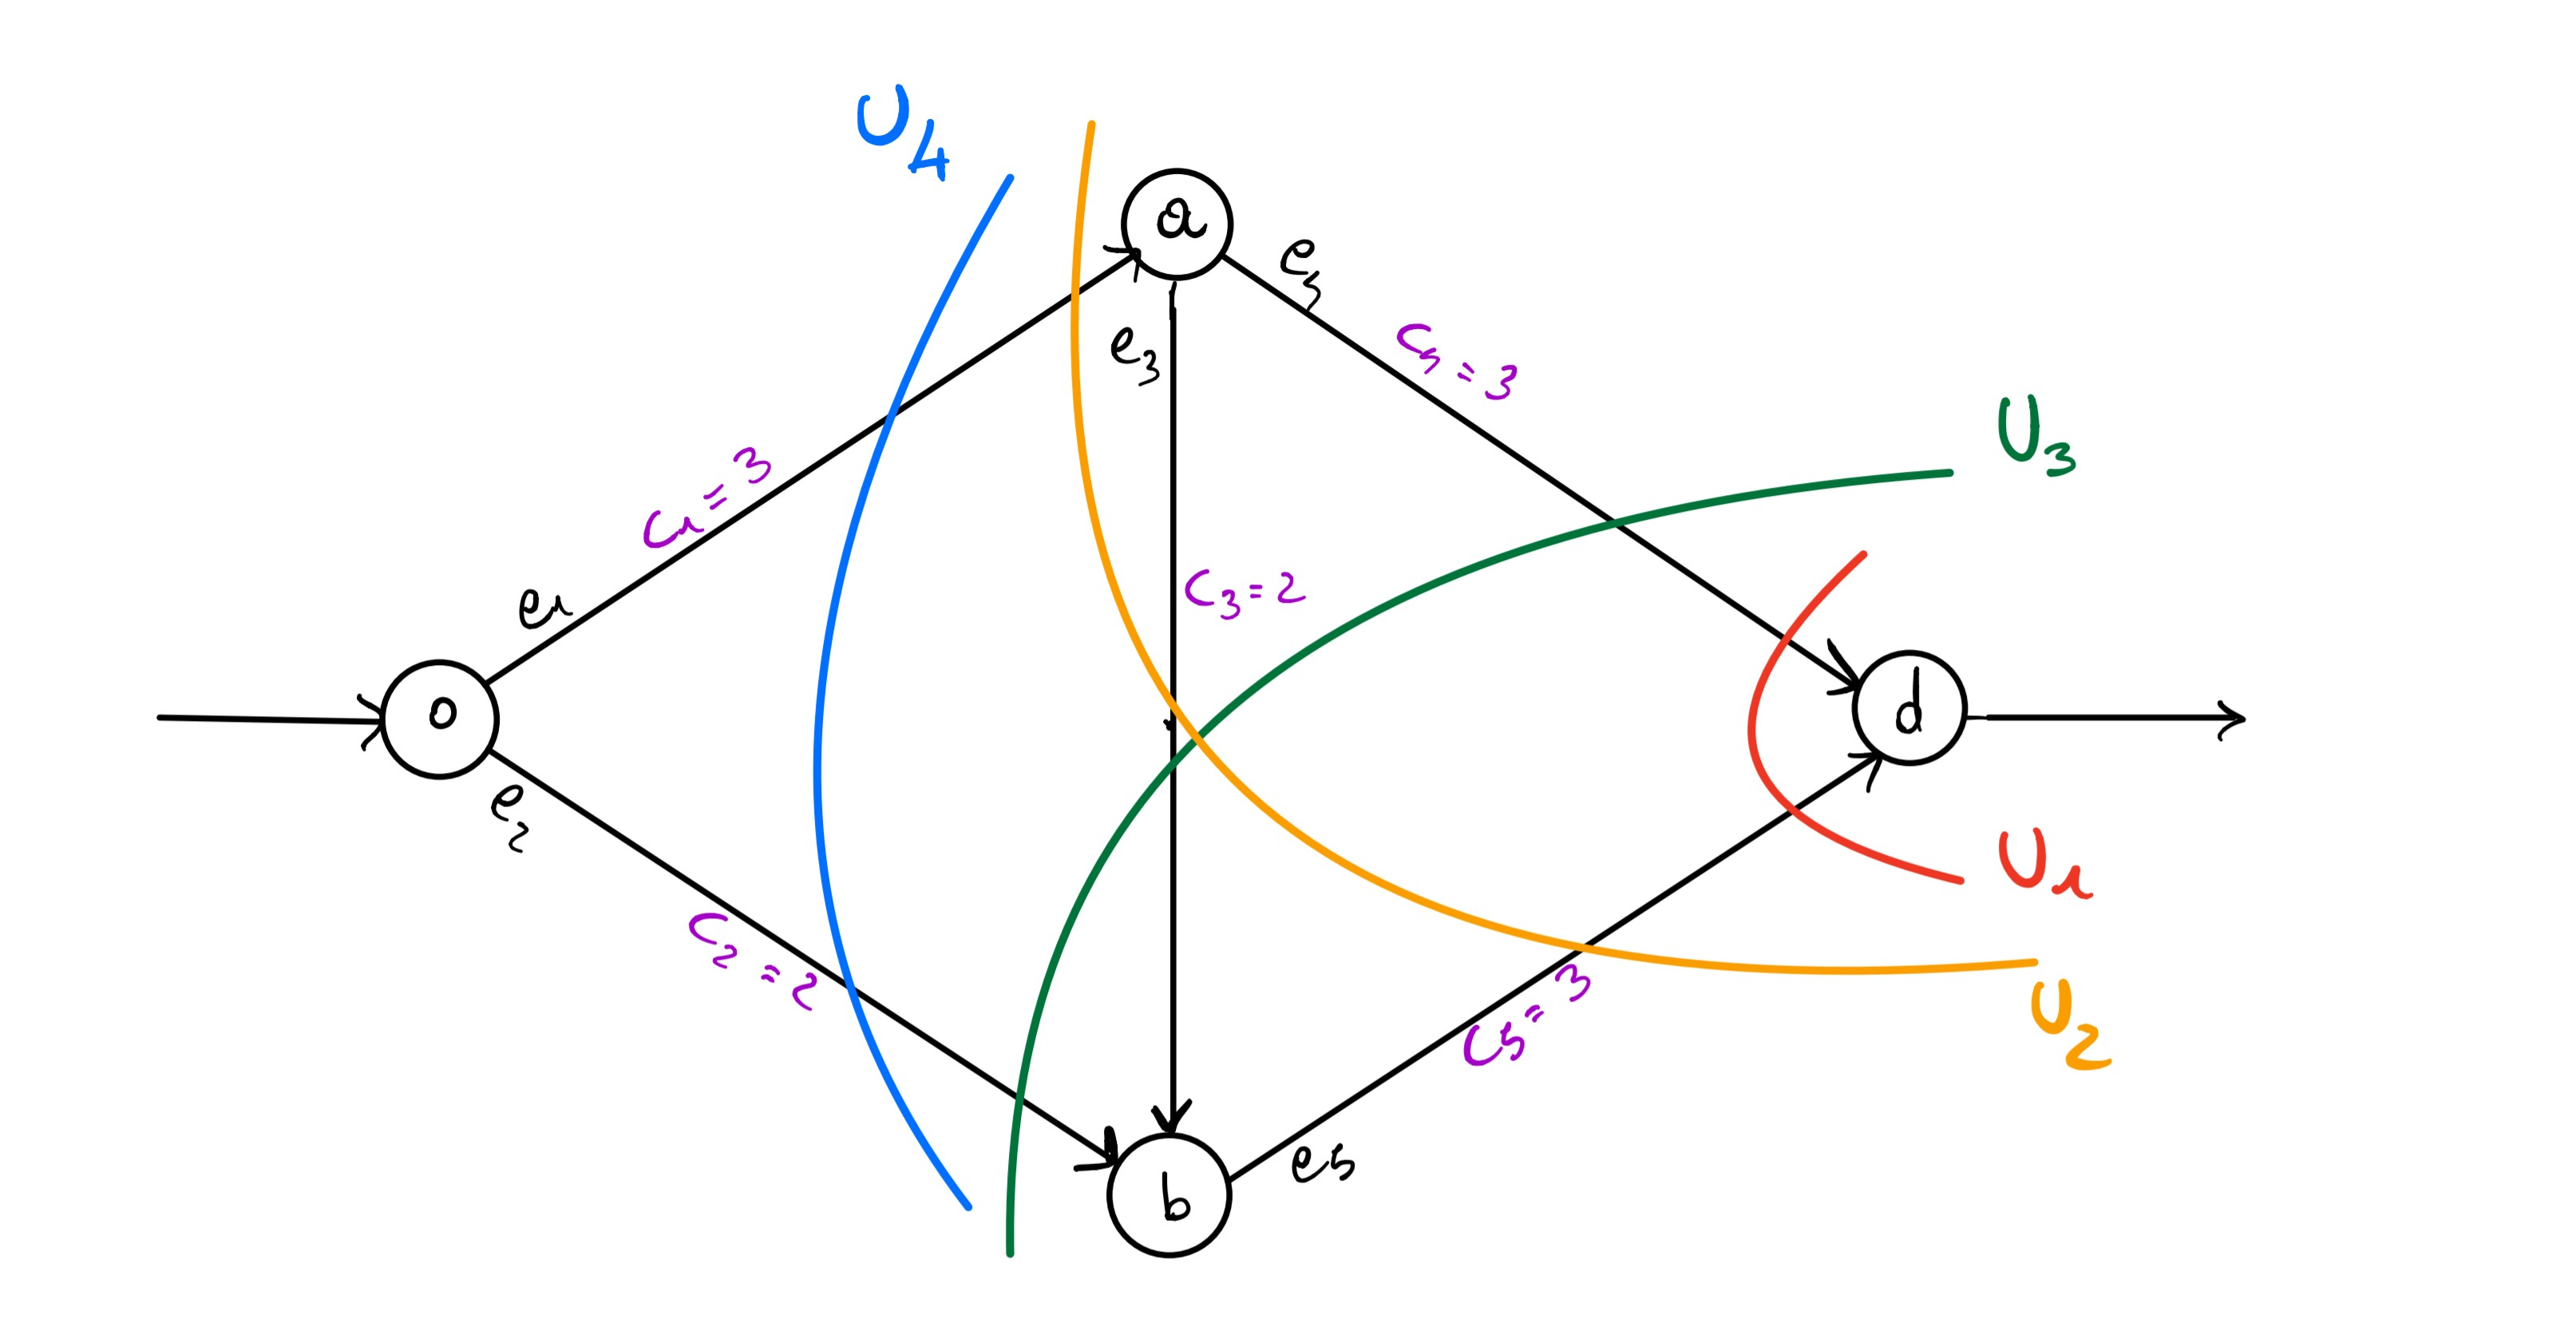
\includegraphics[scale=0.17]{ES1_Fig1.jpg}
  \end{figure}
  Tutti i possibili path \(o-d\) sono i seguenti:

  \begin{description}
    \item[1.] \(p_{(1)}= o -a-d\)
    \item[2.] \(p_{(2)}=o-b-d\) 
    \item[3.] \(p_{(3)}= o-a-b-d\) 
  \end{description}

  I possibili cut e annesse capacità sono:

  \begin{align*}
    U_1 = \{d\}\  && C(U_1)=5 \\
    U_2 = \{a, d\} && C(U_2)=5 \\
    U_3 = \{b,d\} && C(U_3)=7 \\
    U_4 = \{a,b,d\} && C(U_4)=5
  \end{align*}
  
  \begin{alphaparts}
  %----------------------------------------------------------------------------
    \questionpart
    Tutti i possibili colli di bottiglia del grafo hanno capacità pari a 5, quindi per ostruire qualsiasi tipo di flow unitario da \(o\) a \(d\) bisogna eliminare una capacità \(C^*\) tale che
    \begin{equation*}
      C^*<4
    \end{equation*}
%------------------------------------------------------------------------------
    \questionpart
    Dal momento che vale il teorema del \textit{Max Flow - Min Cut}, le due unità di capacità devono essere distribuite in modo tale da aumentare lacapacità del minimo taglio. Poiché ci sono ben tre tagli su 4 che rappresentano un minimo taglio \((U_1, U_2, U_4)\) è necessario aumentare la capacità su archi in comune a questi tre tagli.\\
    Una scelta possibile potrebbe essere quella di aggiungere un'unità di capacità ciascuno agli archi \(e_1\) ed \(e_4\) in modo tale che i tagli risultino:
    
  \begin{align*}
    U_1 = \{d\}\  && C(U_1)=6 \\
    U_2 = \{a, d\} && C(U_2)=6 \\
    U_3 = \{b,d\} && C(U_3)=9 \\
    U_4 = \{a,b,d\} && C(U_4)=6
  \end{align*}

  Aumentando in questo modo il massimo troughput da 5 a 6

%------------------------------------------------------------------------------------
  \questionpart
  Assegnati i seguenti delay a ciascun arco:
  \begin{align*}
    d_1(x)=d_5(x)=x+1, && d_3(x)=1, && d_2(x)=d_4(x)=5x+1
  \end{align*}
  e definendo con \(z_i\) il flusso sull'i-esimo path, si calcola il delay complessivo su ciascun path:
  \begin{align*}
    d_{p_1}&=6z_1+z_3+2 \\
    d_{p_2}&=6z_2+z_3+2 \\
    d_{p_3}&=2z_3+z_1+z_2+3
  \end{align*}

  Si calcola ora l'equilibrio di Wardrop considerando che \(z_1+z_2+z_3=1\) (quindi che \(z_1+z_2=1-z_3\))e che il delay su ciascun path con flusso non nullo deve essere minore di qualsiasi altro delay.

  \begin{align*}
      z_1<0 \Rightarrow  && 6z_1 + z_3 + 2 \leq 2z_3+z_1+z_2+3,  && \Rightarrow z_1 \leq \frac{1}{3}
    \end{align*}

  \begin{align*}
    z_3>0 \Rightarrow && 2z_3+z_1+z_2+3 \leq 6z_1 + z_3 + 2 && \Rightarrow z_1 \geq \frac{1}{3}\\
    && 2z_3+z_1+z_2+3 \leq 6z_2 + z_3 + 2 && \Rightarrow z_2 \geq \frac{1}{3}
  \end{align*}

  \begin{align*}
    z_2>0 \Rightarrow && 6z_2 + z_3 + 2 \leq 2z_3+z_1+z_2+3 && \Rightarrow z_2 \leq \frac{1}{3}\\
  \end{align*}
  
  Queste condizioni implicano che un possibile vettore di flusso che soddisfi le condizioni di Wardrop sia il seguente:

  \begin{equation*}
    z_{\text{Wardrop}} = z_W = \left(\frac{1}{3},\frac{1}{3},\frac{1}{3}\right)
  \end{equation*}

  Il ritardo totale che deriva da questo vettore di flusso è dato da:
  \begin{align*}
    \frac{2}{3}\left(\frac{2}{3}+1 \right) + \frac{5}{9} + \frac{1}{3} + \frac{1}{3} + \frac{5}{9} + \frac{1}{3} + \frac{2}{3}\left(\frac{2}{3}+1 \right) = \frac{13}{3}
  \end{align*}
%-------------------------------------------------------------------------------------
  \questionpart

  Calcolare l'ottimo di sistema equivale a minimizzare il ritardo totale in funzione del flusso su ciascun path \(o\) - \(d\):
  \begin{equation*}
    \min\limits_z (z_1+z_3)(z_1+z_3+1)+(5z_2^2+z_2)+(z_3)+(5z_1^2+z_1)+(z_2+z_3)(z_2+z_3+1)
  \end{equation*}
  Utilizzando la condizione di flusso unitario (\(z_1+z_2+z_3=1\)) si ottiene:
  \begin{eqnarray*}
    \min\limits_z (1-z_2)(2-z_2)+(5z_2^2+z_2)+\\
    +(1-z_1-z_2)+(5z_1^2+z_1)+(1-z_1)(2-z_2)=\\
    \min\limits_z 3(2z_1^2-z_1)+3(2z_2^2-z_2)+5
  \end{eqnarray*}
  Da cui si deduce:
  \begin{align*}
    z_1=\frac{1}{4} && z_2 = \frac{1}{4}
  \end{align*}

  Quindi:

  \begin{equation*}
    z_{\text{Sistema}}=z_S=\left(\frac{1}{4},\frac{1}{4},\frac{1}{2}\right)
  \end{equation*}

  Questa configurazione dei flussi produce un ritardo totale dato da:

  \begin{equation*}
    \frac{3}{4}\left(\frac{3}{4}+1\right)+\frac{1}{4}\left(\frac{5}{4}+1\right)+\frac{1}{2}+\frac{1}{4}\left(\frac{5}{4}+1\right)+\frac{3}{4}\left(\frac{3}{4}+1\right)= \frac{17}{4}
  \end{equation*}
%--------------------------------------------------------------------------------------
  \questionpart
  Il costo totale dell'anarchia è dato dal rapporto tra il il ritardo totale dell'ottimo di sistema e il ritardo totale dell'equilibrio di Wardrop

  \begin{equation*}
    \frac{\frac{13}{3}}{\frac{17}{4}}=\frac{52}{51}
  \end{equation*}
 %------------------------------------------------------------------------------------ 
  \questionpart
  Siano \(f^*_{e_i}\) e \(f^{(w)}_{e_i}\) i flussi su ciascun arco \(e_i\) rispettivamente nella configurazione dell'ottimo di sistema e in quella di equilibrio di Wardrop. Sia il ritardo totale su ciascun arco \(e_i\) definito come \(C_{e_i}(f_e)=d_{e_i}f_{e_i}\). La configurazione ottimale dei pedaggi per ottenere un costo dell'anarchia unitario è la seguente:
  \begin{equation*}
    \omega_{e_i}=C'_{e_i}(f^*_{e_i})-d_{e_i}(f^*_{e_i})=f^*_{e_i}d'_{e_i}(f^*_{e_i})
  \end{equation*} 

  che nel caso specifico si traduce in:

  \begin{align*}
    \omega_{e_1}&=\frac{3}{4} 1=\frac{3}{4}\\
    \omega_{e_2}&=\frac{1}{4} 5=\frac{5}{4}\\
    \omega_{e_3}&=0\\
    \omega_{e_4}&=\frac{5}{4}\\
    \omega_{e_4}&=\frac{3}{4}\\
  \end{align*}

  \end{alphaparts}

  
\section{}%---------------ESERCIZIO 2-----------------------------------
  \begin{alphaparts}
    \questionpart

    La matrice dei pesi \(W\) è la seguente:
    \begin{equation*}
      W=
      \begin{bmatrix}
        a & 1 & 0 & 0 \\
        0 & 0 & 1 & 1 \\
        0 & 0 & 0 & 1 \\
        1 & 1 & 0 & 0
      \end{bmatrix}
    \end{equation*}
    la matrice dei pesi normalizzata è data da:
    \begin{align*}
      \omega=\begin{pmatrix}
        a+1 \\ 2 \\ 1 \\ 2
      \end{pmatrix} && \Rightarrow &&
      P=\begin{bmatrix}
        \frac{a}{a+1} & \frac{1}{a+1} & 0 & 0 \\
        0 & 0 & \frac{1}{2} & \frac{1}{2} \\
        0 & 0 & 0 & 1 \\
        \frac{1}{2} & \frac{1}{2} & 0 & 0
      \end{bmatrix}
    \end{align*}

    Di conseguenza il laplaciano è dato da:
    \begin{equation*}
      L=D-W= \begin{bmatrix}
        1 & -1 & 0 & 0 \\
        0 & 2 & -1 & -1 \\
        0 & 0 & 1 & -1 \\
        -1 & -1 & 0 & 2 \\
      \end{bmatrix}
    \end{equation*}
    %---------------------------------------------------------------------------------
    \questionpart
    La dinamica di opinione di French-De Groot è data da:
    \begin{equation*}
      x(t+1)=Px(t)
    \end{equation*}
    dove \(x(t)=(x_1(t),x_2(t),x_3(t),x_4(t))\) e \(x_i(t)\) rappresenta il valore dell'opinione del nodo \(i\) al tempo \(t\).

    %----------------------------------------------------------------------------------

    \questionpart
    Affinchè l'opinione su \(\mathcal{G}\) converga ad un consenso il grafo deve essere fortemente connesso ed aperiodico. Date le ridotte dimensioni del grafo è possibile verificare queste due proprietà manualmente, notando che è possibile raggiungere qualsiasi nodo a partire da qualsiasi posizione sul grafo e che ad esempio il nodo 4 ha un ciclo di lunghezza 2 e un altro di lunghezza 3. Connessione ed aperiodicità sono indipendenti dal valore di \(a\) pertanto vale:
    \begin{align*}
      \lim\limits_{t \rightarrow \infty} x(t)=\pi ' x(0) && \forall a\geq 0
    \end{align*}

    Dal momento che \(\mathcal{G}\) è bilanciato la misura di probabilità invariante \(\pi \) è proporzionale al vettore \(\omega\). In particolare:
    \begin{equation*}
      \pi = \frac{\omega}{\mathbb{1}'\omega}=\begin{pmatrix}
        \frac{a+1}{a+6} & \frac{2}{a+6} & \frac{1}{a+6} & \frac{2}{a+6}
      \end{pmatrix}'
    \end{equation*}

    Pertanto il valore del consenso converge ad un valore finito fintanto che \(a \neq -6\), condizione automaticamente verificata dal momento che \(a \geq 0\)
    %--------------------------------------------------------------------------
    \questionpart

    Nel caso particolare in cui \(a=0\) si ha:
    \begin{equation*}
      \pi = \begin{pmatrix}
        \frac{1}{6} & \frac{1}{3} & \frac{1}{6} & \frac{1}{3}
      \end{pmatrix}'
    \end{equation*} 

    Per cui, date le condizioni iniziali \(x(0)\), il consenso raggiunge il seguente valore: 
    \begin{align*}
      \lim\limits_{t \rightarrow \infty} x_i(t)=\pi ' x(0) = \frac{1}{3} && \forall i = 1 \dots 4
    \end{align*}

    %----------------------------------------------------------------------------------
    \questionpart
    Poiché il consenso viene raggiunto \(\forall a \geq 0 \), date le condizioni iniziali \(x(0)\), vale la seguente:
    \begin{equation*}
      \lim\limits_{t \rightarrow \infty} x_1(t)=\pi ' x(0) = \frac{1}{a+6}(-a+1+2-1+2) = \frac{2-a}{a+6}
    \end{equation*}

    segue quindi che:
    \begin{align*}
      \lim\limits_{t \rightarrow \infty} x_1(t) \leq 0 &&\Rightarrow&& \frac{2-a}{a+6} \leq 0 && \Rightarrow && a \geq 2 
    \end{align*}

    %-------------------------------------------------------------------------------

    \questionpart

    Date \(x_i(0)\) variabili aleatorie indipendenti e identicamente distribuite tali che \(Var(x_i(0))=1 \text{ }\forall i =1 \dots 4\), vale la seguente:

    \begin{equation*}
      \lim\limits_{t \rightarrow \infty} x_1(t) = \frac{a+1}{a+6}x_1(0)+\frac{2}{a+6}x_2(0)+ \frac{1}{a+6}x_3(0)+\frac{2}{a+6}x_4(0)
    \end{equation*}

    Poiché le variabili sono i.i.d. e \(Var(x_i(0))=1 \text{ }\forall i =1 \dots 4\) vale:

    \begin{gather*}
      Var\left(\lim\limits_{t \rightarrow \infty} x_1(t)\right) = \left(\frac{a+1}{a+6}\right)^2Var(x_1(0))+\left(\frac{2}{a+6}\right)^2Var(x_2(0))+\\+ \left(\frac{1}{a+6}\right)^2Var(x_3(0))+\left(\frac{2}{a+6}\right)^2Var(x_4(0)) = \\
      = \frac{a^2 + 2a + 10}{(a+6)^2}=v(a)
    \end{gather*}

    Essendo \(v(a)\) una funzione convessa, si verifica facilmente che raggiunge un minimo per:
    \begin{equation*}
      a= \frac{4}{5}
    \end{equation*}
    Che rappresenta il valore di \(a\) per cui viene minimizzata la varianza del consenso.

  \end{alphaparts}
  






\section{}%---------------ESERCIZIO 3 ------------------------------------------
  

\section*{Using the \texttt{section} Macro}
  The starred \texttt{section*} works as well.

  \lipsum[11]
% Sometimes questions get separated from their bodies. Use a \newpage to force
% them to wrap to the next page.

  
% Use \renewcommand{\questiontype}{<text>} to change what word is displayed
% before numbered questions
\renewcommand{\questiontype}{Task}
\end{document}
